
\section{Manipulação de Device drivers}
Aplicações executados no \textit{User space} interagem com o hardware atraves de funções suportadas
pelo kernel. Assim, geralmente essas funções são voltadas para leitura e escrita de arquivos, dado que um
device driver, do ponto de vista do usuário, são vistos como arquivos. No lado do kernel, também
existem funções análogas voltadas para interação direta com hardware de modo que a informação deste
possa ser enviado as aplicações no espaço de usuário. A imagem a seguir apresenta uma relação de algumas
funções do espaço do usuário e no espaço do kernel.

\begin{figure}[H]
  \centering
  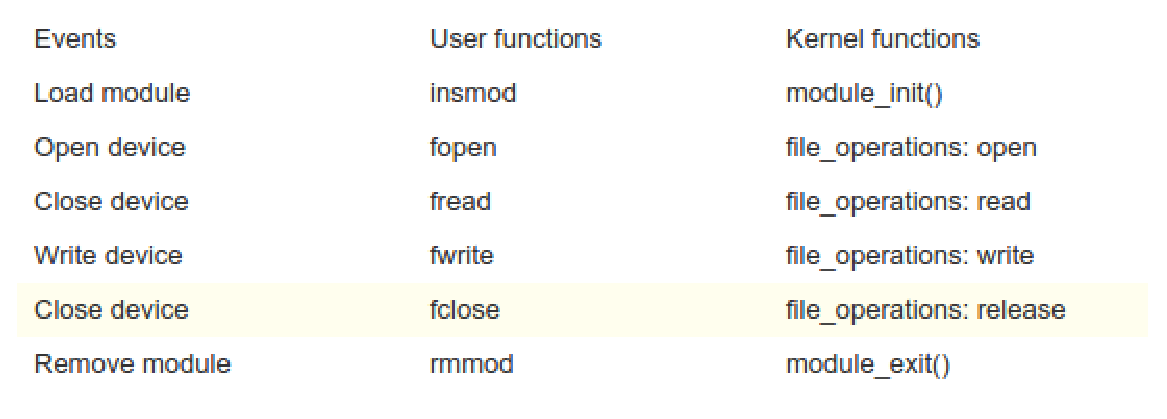
\includegraphics[width=0.9\textwidth]{figure/tabela.eps}
  \caption{ Eventos de \textit{device drivers} associados com funções de interface entre o \textit{kernel} e \textit{user space} }.
  \label{fig:usblinux}
\end{figure}

Assim, por exemplo no espaço do usuário, para instalar o módulo é feita a chamada a função \textbf{insmod} passando
como argumento o módulo a ser carregado. Em seguida, no lado do kernel é chamada a função \textbf{module\_init()} de
modo que assim alguma tarefas , como reservar memória ram e portas de entrada e saída são executadas.
Por outro lado, para a remoçao de um módulo é feita a chamada de função \textbf{rmmod} passando como argumento
o módulo a ser removido, no lado do \textit{kernel} é chamada a função \textbf{module\_exit()}, liberando assim os recursos
de hardware alocados anteriormente. O codigo a seguir apresenta um \textit{hello word} tipico de \textit{device driver}.

\lstset{style=shell}
\lstinputlisting[language=Bash, label=code:hello, caption="Um exemplo de Hello World de device driver"]{code/hello.c}

Nas linhas de 1 a 3 são incluídas as bibliotecas utilizadas para uso de funções necessárias para 
construção de device drivers. Os métodos \textbf{hello\_init} e \textbf{hello\_exit} são executados quando um módulo 
é instalado e removido respectivamente. Destaca-se que esse métodos são passado para funções \textbf{ module\_init}
e \textbf{module\_exit} como argumento para que os mesmos sejam executados nessas operações ( instalação e 
remoção de módulos). Outro destaque é uso da função \textit{printk}, essa função possui ação semelhante a do \textit{printf}, 
entretanto ela típica do \textit{kernel} e imprime apenas nos arquivos de \textit{log} do sistema.


\section{Descrição da Solução}

A solução proposta consta com a leitura de um device driver para um mouse USB.
No estado atual do driver é possível reconhecer uma ação provida pelo mouse.
Essa ação pode ser um click ou a movimentação do mouse que causa uma interrupção
utilizando urb.

Começando pela inicialização do driver. Como mostrado na seção anterior, os módulos
devem conter uma simples declaração das funções de inicialização e remoção de um
módulo kernel. 

\lstset{style=shell}
\lstinputlisting[firstline=63,lastline=85,language=C, label=code:init, caption="Funções init e exit"]{../../labs/driver/mouse.c}

Nas duas funções apresentadas no código \ref{code:init} de \textit{init e exit} contém, respectivamente,
o registro e o desregistro do \textit{driver} USB. Para a declaração de um \textit{driver} é necessário utilizar
o construtor \textit{usb\_driver} contida na biblioteca linux/usb.h

\lstset{style=shell}
\lstinputlisting[firstline=44,lastline=52,language=C, label=code:usbdriver, caption="Struct de usb\_driver."]{../../labs/driver/mouse.c}

Nessa estrutura são declaradas as principais funções utilizadas pela api USB do kernel. São elas:
\textit{name}, que registra o driver com um nome (no caso, está sendo representado pelo nome do proprío
arquivo do driver); \textit{id\_table}, onde contém as informações sobre quais os dispositívos suportados
pelo \textit{driver} usb; \textit{probe}, é chamado quando um novo dispositívo é inserido; \textit{disconnect}, é chamado
quando um dispositivo é removido. Com isso nos temos a estrutura principal do nosso \textit{driver}.
Lembrando que todos os argumentos desse quatro componentes já foram declarados anteriormente.

O \textit{id\_table} é uma estrutura macro que define quais os dispositívos suportados pelo drive
através dos identificadores VENDOR e PRODUCT que podem ser recuperados utilizando o comando
\textit{lsusb}. A declaração segue o modelo:

\lstset{style=shell}
\lstinputlisting[firstline=26,lastline=32,language=C, label=code:usbdriver, caption="Struct de usb\_device\_id."]{../../labs/driver/mouse.c}

Para compilar este driver, utilizou-se o Makefile descrito no código \ref{code:makefile}. O
código foi alterado para que seja possível compilar mais de um driver disponível na mesma pasta.

\lstset{style=shell}
\lstinputlisting[language=Bash, label=code:makefile, caption="Makefile utilizado para compilação de drivers."]{../../labs/driver/Makefile}

No caso da macro \textit{obj-m:}, deve-se passar o arquivo referente ao compilado do \textit{driver}, no nosso
caso, o arquivo onde contém o código do mouse se chama \textit{mouse.c}, logo, a macro poderia ser
declarada estaticamente utilizando \textit{obj-m: mouse.o}. Após isso, o principal é a função \textit{compile}
que define como é feito a compilação. No caso estamos utilizando a versão padrão utilizada
pelo sistema operacional com o argumento \textit{shell uname \-r} que retorna o nome exato da versão.
Fique atento quanto a versão do kernel, em algumas há funções depreciadas ou que trocaram
de nome, portanto sempre consulte a documentação oficial.

Neste ponto é possível inicializar o \textit{driver} com a função \textit{insmod}. No caso dos USBs, caso um
\textit{driver} tiver prioridades quanto ao dispositívo ele será carregado primeiro. Portanto, é
necessário, para \textit{drivers} de mouse usb, remover o \textit{driver} padrão que é carregado quando
o dispositívo é plugado. Nos testes utilizados nesse projeto, o \textit{driver} padrão para
dispositívos de interação humana (mouse, teclado, etc) é o \textit{usbhid}, remova-o caso
necessário.


Aprofundando a função \textit{probe} do nosso \textit{driver} nos temos o registro da interface e declaração do URBs
(mais explicado seção \ref{driverusb}). Aqui, esse registro significa dizer para o USB Core com qual
interface nos estamos trabalhando. No caso da implementação estamos nos referendo a uma interface
de interrupção que são próprias pra lidar com recebimento e envio de dados para o dispositivo.
\lstset{style=shell}
\lstinputlisting[language=C,firstline=158,lastline=185, label=code:urbs, caption="Declaração de URBs."]{../../labs/driver/mouse.c}

\lstset{style=shell}
\lstinputlisting[language=C,firstline=143,lastline=158, label=code:reg, caption="Registro da interface do \textit{device}."]{../../labs/driver/mouse.c}

Todas as informações são armazenadas em uma struct interna do código que guarda a referencia
de todos os itens relacionados ao dispositívo, como \textit{endpoint address, buffers, interfaces, etc}.

\lstset{style=shell}
\lstinputlisting[language=C,firstline=52,lastline=63, label=code:reg, caption="Struct interna ao código."]{../../labs/driver/mouse.c}

Dentro da função \textit{probe} também há a declaração das URBs, ou blocos de comunicação.
Geralmente os URBs são declarados nas funções de leitura e escrita
que definem os pacotes de comunicação urbs que serão trasmitidos para o dispositívo.
Por problemas de implementação, essa declaração de ubs não está adequada ao necessário
para a proposta.

\lstset{style=shell}
\lstinputlisting[language=C,firstline=158,lastline=185, label=code:urbs, caption="Declaração de URBs."]{../../labs/driver/mouse.c}

Na utilizaçãod o URBs, é necessário: alocar memória para a estrutura, isso é feito no
espaço do kernel; definir o buff para alocar as informações a serem transmitidas;
initicializar o urb; submeter o urb para o USB Core que irá enviar para o dispositívo.
Com a conclusão desses passos, a comunicação com o urb está pronta. Um importante item
é a função \textit{usb\_fill\_int\_urb}, nela é declarada não apenas o \textit{endpoint} de comunicação
como também a função a ser chamada quando ocorre uma interrupção feita pelo dispositivo.
No caso estamos declarando a função \textit{mouse\_callback} que contem um simples \textit{printk} para
demonstrar a ação do dispositivo.

\lstset{style=shell}
\lstinputlisting[language=C,firstline=88,lastline=105, label=code:callback, caption="Callback do urb."]{../../labs/driver/mouse.c}

Com essa estrutura, é possível reconhecer a primeira ação do dispositivo mouse USB.
Há problemas técnicos quanto a essa implementação, não é possível reconhecer
mais de uma ação. Com isso é necessário realizar outras melhorias para que isso
seja possível.

Sempre na construção de um módulo kernel, é necessário desregistrar o dispositivo.
Isso é realizado com a função \textit{mouse\_disconnect()}. É uma simples utilização das
funções da api USB Core. Isso garante que o dispositivo não entre em conflito
caso ele seja inserido novamente.

\lstset{style=shell}
\lstinputlisting[language=C,firstline=191,lastline=207, label=code:urbs, caption="Função de disconnect."]{../../labs/driver/mouse.c}

Neste ponto, nós temos um \textit{driver} específico para um mouse USB que reconhece a primeira
ação do mouse.

Nos mouses e teclados, por exemplo, é comum a presença dos \textit{endpoint} de interrupção IN.
O modelo de declaração de urbs irá seguir os mesmos passos, entretanto com a utilização
de funções específicas para os tipos \textit{bulk, control e isochronous}.

